% !TeX spellcheck = it_IT
\section{Alexandrov Moving Planes Method}
% --- Moving planes ---
\begin{frame}{Alexandrov Moving Planes Method}{Cenni storici}
	\begin{itemize}
		\item Tecnica per dimostrare la simmetria delle soluzioni a PDE ellittiche e paraboliche. 
		\item<2-> Introdotto da Alexandrov per caratterizzare la sfera 
		\begin{itemize}
			\item Alexandrov A.D.; \textit{A characteristic property of spheres}, 1962
		\end{itemize}
		\item<3-> Serrin e da Gidas-Ni-Nirenberg lo applicano a soluzioni di PDE ellittiche di natura non-geometrica
		\begin{itemize}
			\item Serrin J.; \textit{A symmetry problem in potential theory}, 1971
			\item Gidas B., Ni W.M., Nirenberg L.; \textit{Symmetry and Related Properties via the Maximum Principle}, 1979
		\end{itemize}
	\end{itemize}
\end{frame}

% --- Moving planes ---
\begin{frame}{Alexandrov Moving Planes Method}{Il metodo in breve}
	\begin{columns}
		% First column
		\column{.72\textwidth}
		\begin{itemize}
			\item Rifletto una soluzione rispetto a una famiglia di piani paralleli
			\item<2-> Considero il piano dove c'è ``per la prima volta'' \textit{tangenza interna} dei grafici
			\item<3-> Applico il principio del massimo alla differenza di soluzione e riflessione
			\item<4-> Deduco che la funzione è simmetrica rispetto a quel piano. Per arbitrarietà della direzione, ho simmetria sferica
		\end{itemize}
		% Second column
		\column{.28\textwidth}
		\begin{figure}
			\begin{center}
				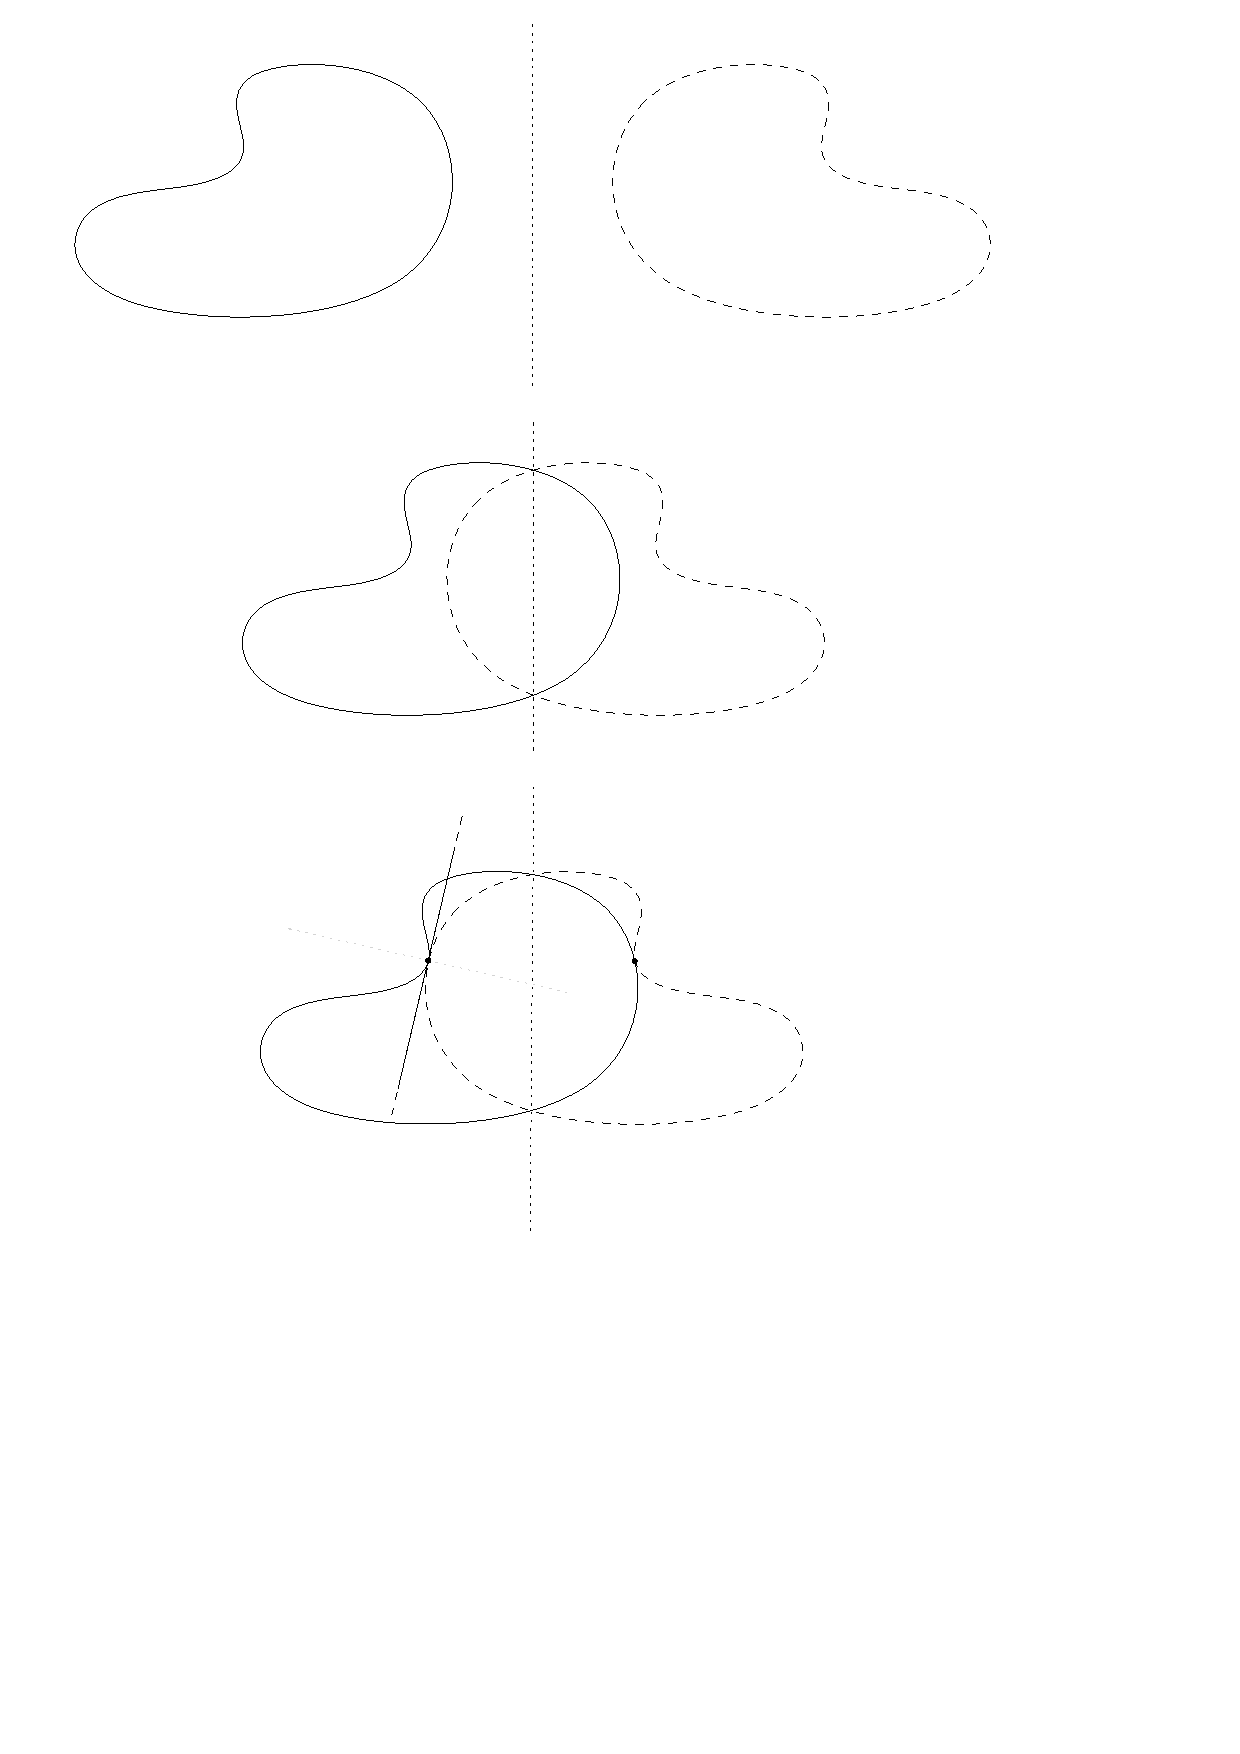
\includegraphics[width=\textwidth]{6_method moving planes}
				\caption{}
			\end{center}
		\end{figure}
	\end{columns}
\end{frame}

\section{Il risultato di Chow-Gulliver}


% --- Equazione di cui ci occupiamo ---
\begin{frame}{Equazione di cui ci occupiamo}{}
	\begin{block}{Flusso geometrico di cui ci occupiamo}
		\begin{align*}
			\frac{\partial X_t}{\partial t} = - F(\kappa_1(x), \dots , \kappa_n(x)) \nu
		\end{align*}
		dove $\nu$ è il vettore normale, $\kappa_i$ le curvature principali e $F$ una funzione simmetrica tale che 
		\begin{align*}
			\frac{\partial F}{\partial \kappa_i} > 0 \mathrm{\; for \; all } \; i=1,\dots, n
		\end{align*}
	\end{block}
	\begin{block}{}<2->
		La condizione sulle derivate di $F$ è equivalente a dire che questa sia una \textbf{equazione parabolica} (non-lineare). In particolare, possiamo applicare il principio del massimo e l'Hopf Boundary Point Lemma alla differenza di due soluzioni. Inoltre, la parabolicità garantisce l'esistenza per tempi piccoli.
	\end{block}
\end{frame}



% --- Riflessione stretta ---
\begin{frame}{Riflessione stretta}{Definizione}
	\begin{block}{Riflessione stretta}
		 Possiamo riflettere $X : M^n \rightarrow R^{n+1}$ strettamente rispetto a $\pi$ se entrambe le seguenti cose sono vere:
		 \begin{itemize}
		 	\item La riflessione di $X$ rispetto a $\pi$ nel semispazio delimitato da $\pi$ resta dentro l'altra metà di $X$, toccandosi solo sul piano
		 	\item A tutti i punti sul piano, $X$ e la sua riflessione rispetto a $\pi$ non hanno lo stesso vettore normale su $\pi$
		 \end{itemize}
	\end{block}
\end{frame}


% --- Cosa non deve succedere ---
\begin{frame}{Riflessione stretta}{Cosa non deve succedere}
	\begin{columns}
		% First column
		\column{.5\textwidth}
		\begin{figure}
			\begin{center}
				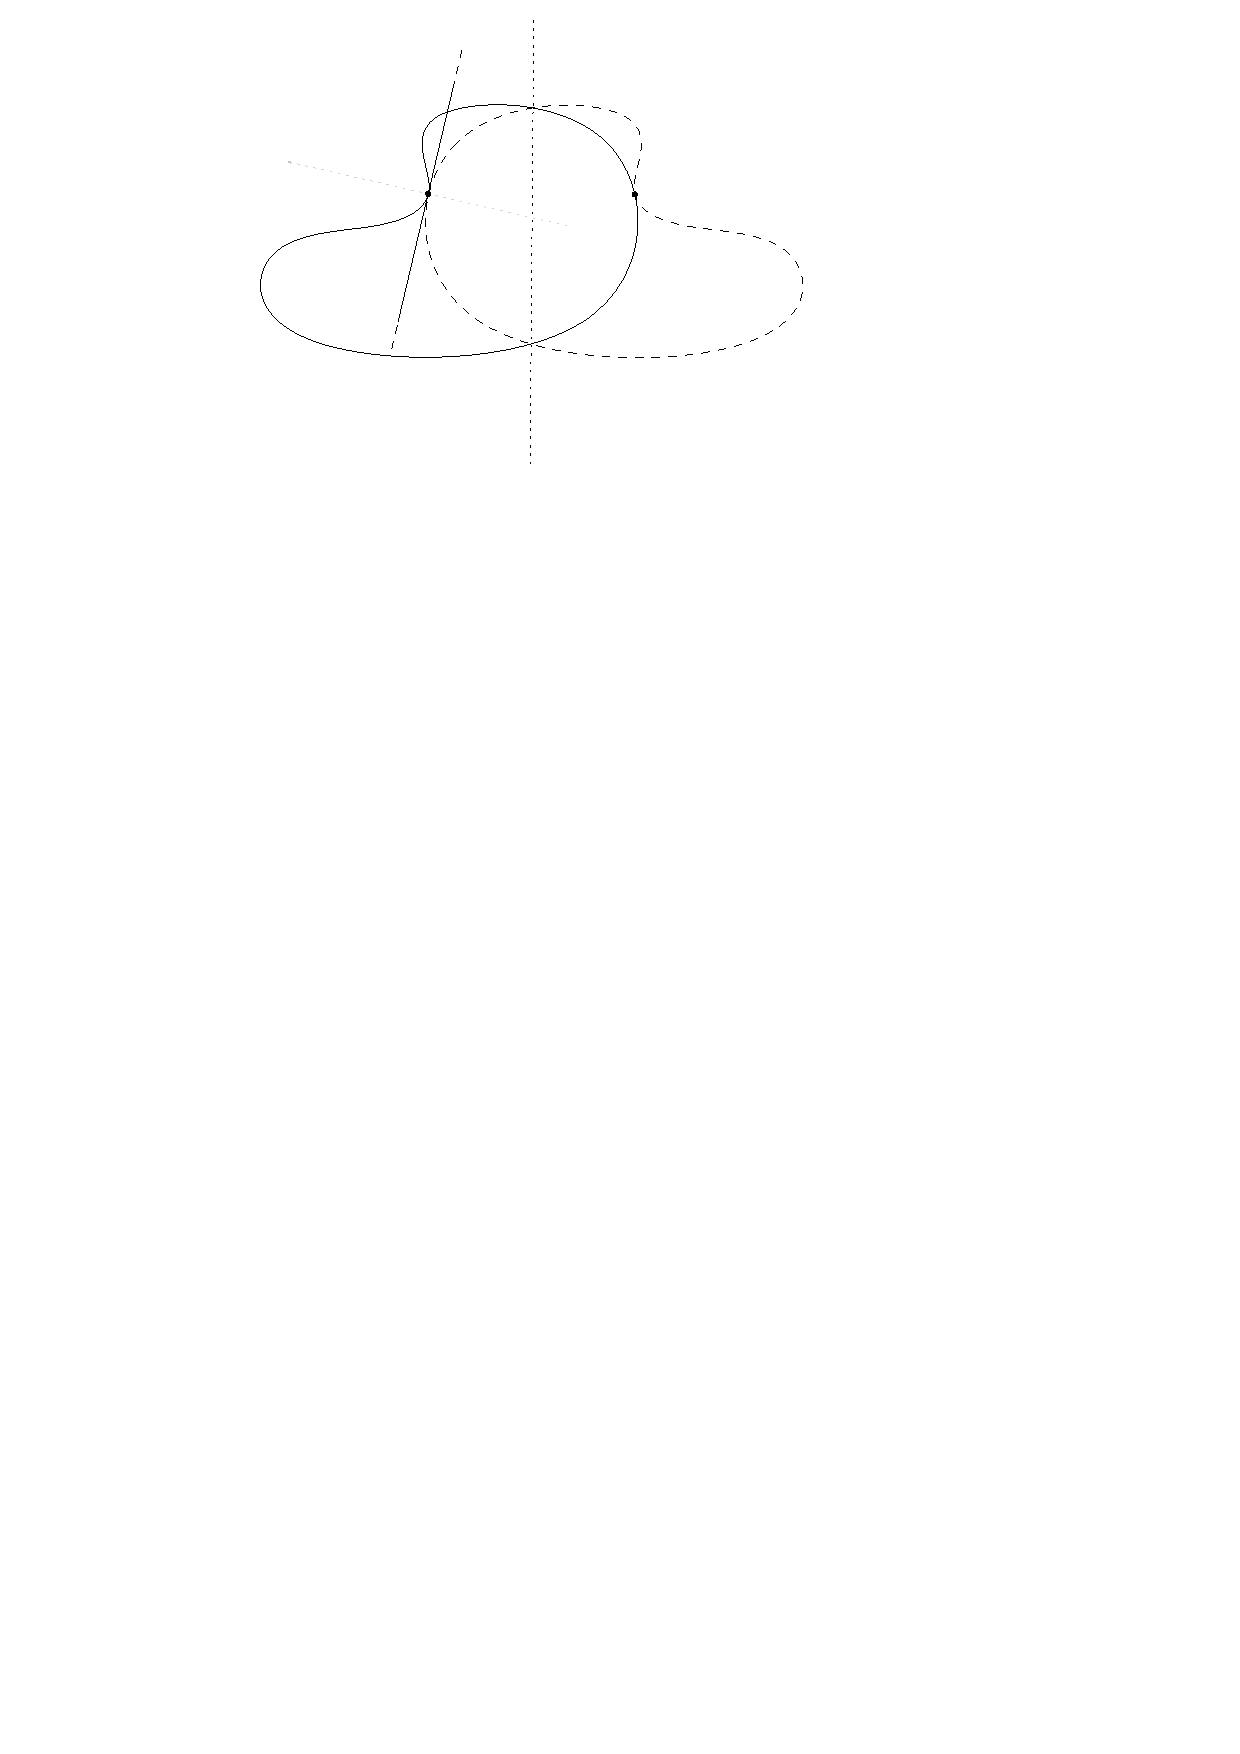
\includegraphics[width=0.8\textwidth]{8_interior_contact}
				\caption{Esempio di contatto interno}
			\end{center}
		\end{figure}
		% Second column
		\column{.5\textwidth}
		\begin{figure}
			\begin{center}
				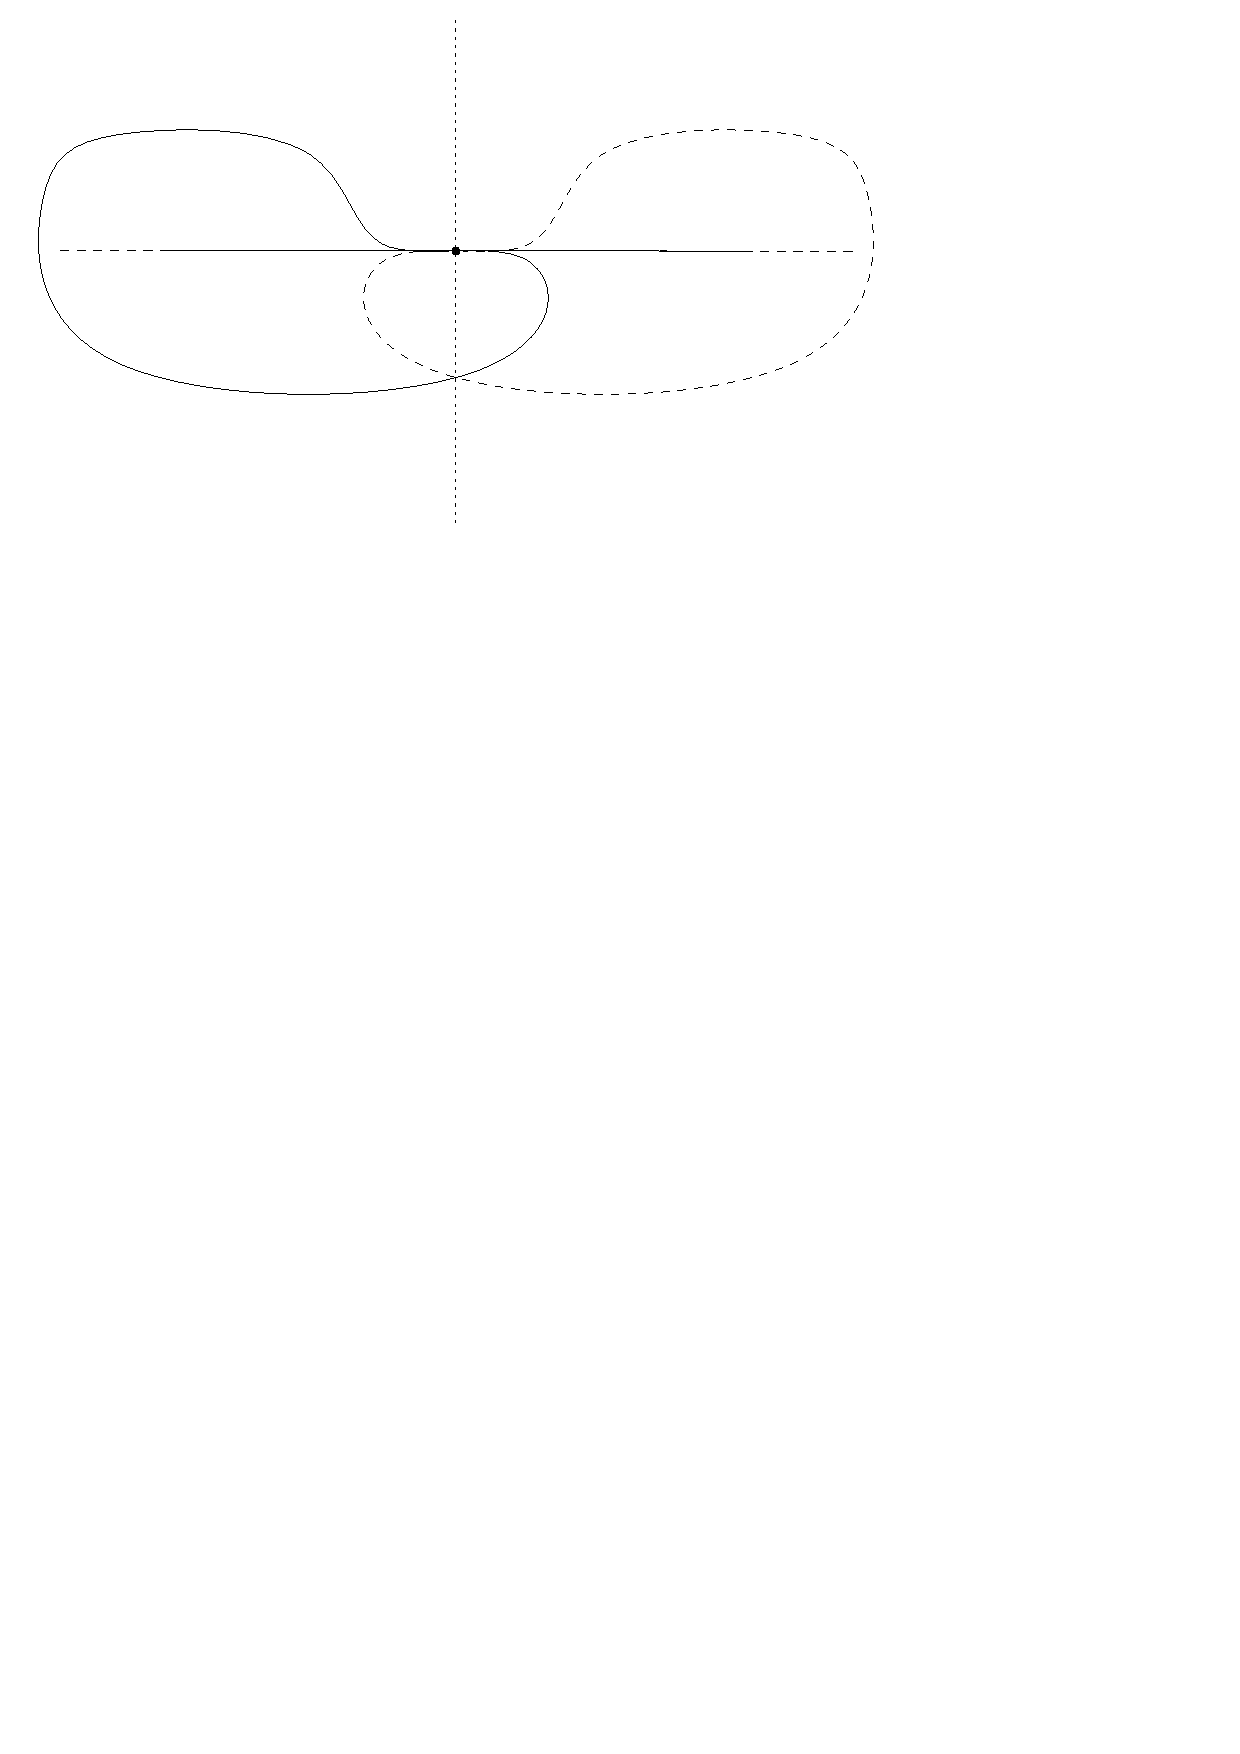
\includegraphics[width=\textwidth]{9_boundary_contact}
				\caption{Esempio di contatto al bordo}
			\end{center}
		\end{figure}
	\end{columns}
\end{frame}




% --- Il teorema di Chow e Gulliver ---
\begin{frame}{Il teorema di Chow e Gulliver}{}
	\begin{block}{Teorema (Chow-Gulliver)}
		Data una soluzione del flusso che stiamo considerando, se possiamo riflettere il dato iniziale $X_0$ strettamente rispetto ad un piano $\pi$, allora possiamo riflettere $X_t$ strettamente rispetto a $\pi$ per ogni $t\in [0,T)$ (intervallo in cui è definita la soluzione). 
	\end{block}
	\begin{block}{}<2->
		\textbf{Interpretazione intuitiva}: i piani rispetto a cui posso riflettere \textit{aumentano} nel tempo, per cui la varietà diventa \textit{più simmetrica} e tonda. 
	\end{block}
\end{frame}